% Template created by Karol Kozioł (www.karol-koziol.net) for ShareLaTeX

\documentclass[a4paper,9pt]{extarticle}
\usepackage[utf8]{inputenc}
\usepackage[T1]{fontenc}
\usepackage{graphicx}
\usepackage{xcolor}
\usepackage{tikz}

\usepackage{amsmath,amssymb,textcomp}
\everymath{\displaystyle}

\usepackage{times}
\renewcommand\familydefault{\sfdefault}
\usepackage{tgheros}
\usepackage[defaultmono,scale=0.85]{droidmono}

\usepackage{multicol}
\setlength{\columnseprule}{0pt}
\setlength{\columnsep}{20.0pt}

% Style for coding: Starts %
\usepackage{listings}
\usepackage{color}

\definecolor{dkgreen}{rgb}{0,0.6,0}
\definecolor{gray}{rgb}{0.5,0.5,0.5}
\definecolor{mauve}{rgb}{0.58,0,0.82}

\lstset{frame=tb,
  language=Python,
  aboveskip=3mm,
  belowskip=3mm,
  showstringspaces=false,
  columns=flexible,
  basicstyle={\small\ttfamily},
  numbers=none,
  numberstyle=\tiny\color{gray},
  keywordstyle=\color{blue},
  commentstyle=\color{dkgreen},
  stringstyle=\color{mauve},
  breaklines=true,
  breakatwhitespace=true,
  tabsize=3
}

% Style for coding: Ends %

\usepackage{geometry}
\geometry{
a4paper,
total={210mm,297mm},
left=10mm,right=10mm,top=10mm,bottom=15mm}

\linespread{1.3}

% custom title
\makeatletter
\renewcommand*{\maketitle}{%
\noindent
\begin{minipage}{0.65\textwidth}

\begin{tikzpicture}
\node[rectangle,rounded corners=6pt,inner sep=10pt,fill=blue!50!black,text width= 0.95\textwidth] {\color{white}\Huge \@title};
\end{tikzpicture}
\end{minipage}
\hfill
\begin{minipage}{0.25\textwidth}
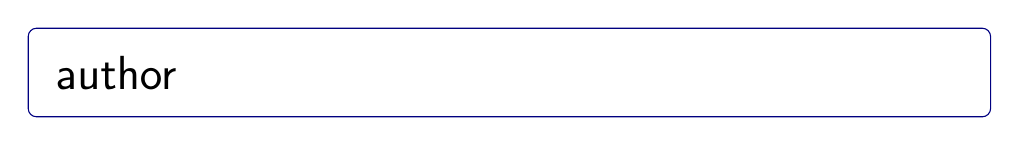
\begin{tikzpicture}
\node[rectangle,rounded corners=3pt,inner sep=10pt,draw=blue!50!black,text width= 0.95\textwidth] {\LARGE \@author};
\end{tikzpicture}
\end{minipage}
\bigskip\bigskip
}%
\makeatother

% custom section
\usepackage[explicit]{titlesec}
\newcommand*\sectionlabel{}
\titleformat{\section}
  {\gdef\sectionlabel{}
   \normalfont\sffamily\Large\bfseries\scshape}
  {\gdef\sectionlabel{\thesection\ }}{0pt}
  {
\noindent
\begin{tikzpicture}
\node[rectangle,rounded corners=3pt,inner sep=4pt,fill=blue!50!black,text width= 0.95\columnwidth] {\color{white}\sectionlabel#1};
\end{tikzpicture}
  }
\titlespacing*{\section}{0pt}{15pt}{10pt}


% custom footer
\usepackage{fancyhdr}
\makeatletter
\pagestyle{fancy}
\fancyhead{}
\fancyfoot[C]{\footnotesize \textcopyright\ \@date\ \ \@author}
\renewcommand{\headrulewidth}{0pt}
\renewcommand{\footrulewidth}{0pt}
\makeatother

\title{Python for JAVA Developers: Basics V 0.1}
\author{By Akash Panchal}
\date{2018}

\begin{document}

\maketitle
\begin{multicols*}{2}

\section{Basic Syntax}
\subsection{End of Statements}
Unlike Java to end a statement in Python, don't have to type in a semicolon, you simply press \boxed{Enter}.
\begin{lstlisting}
message1 = 'Hello World!'
message2 = "Python gives no missing semicolon error!"

# Instead of System.out.print, we use print
print message1 # print 'Hello World!' on the console output
print "Hello Python!"
\end{lstlisting}


\section{Data Types}
Python sets the variable type based on the value that is assigned to it. Unlike more riggers languages, Python will change the variable type if the variable value is set to another value

\begin{lstlisting}
var = 123 # This will create a number integer assignment
var = 'john' # the `var` variable is now a string type.
\end{lstlisting}

\subsection{Numbers}
Most of the time using the standard Python number type is fine. Python will automatically convert a number from one type to another if it needs.

\begin{center}
 \begin{tabular}{||c c c c||}
 \hline
 Type & Java & Python & Description \\ [0.5ex]
 \hline\hline
 int & int a = 11 & a = 11 & Signed Integer\\
 \hline
 long & long a = 1712L & a = 1712L & (L) Long integers\\
 \hline
 float & float a = 19.91 & a = 19.91 & 	(.) Floating point values\\
 \hline
 complex & - - - & a = 3.14J & (J) integer [0 to 255]\\
 \hline
\end{tabular}
\end{center}

\subsection{String}
Create string variables by enclosing characters in quotes. Python uses single quotes \boxed{'} double quotes \boxed{"} and triple quotes \boxed{"""} to denote literal strings. Only the triple quoted strings \boxed{"""} will automatically continue across the end of line statement.

\begin{lstlisting}
firstName = 'Jane'
lastName = "Doe"
message = """This is a string that will span across multiple lines. Using newline characters and no spaces for the next lines."""
\end{lstlisting}

\subsection{List}
Lists are a very useful variable type in Python. A list can contain a series of values. List variables are declared by using brackets [ ] following the variable name.

\begin{lstlisting}
A = [] # This is a blank list variable
B = [1, 23, 45, 67] # creates an initial list of 4 numbers.
C = [2, 4, 'john'] # can contain different variable types.
\end{lstlisting}

\subsection{Tuple}
Tuples are a group of values like a list and are manipulated in similar ways. But, tuples are fixed in size once they are assigned.

\begin{lstlisting}
myGroup = ('Lion', 'Tiger', 'Elephant', 'Giraffe')
\end{lstlisting}

\subsection{Dictionary}
Dictionaries in Python are lists of \boxed{Key}:\boxed{Value} pairs. This is a very powerful datatype to hold a lot of related information that can be associated through \boxed{keys}.

\begin{lstlisting}
room_num = {'john': 121, 'tom': 307}
room_num['john'] = 432  # set the value associated with the 'john' key to 432
print (room_num['tom']) # print the value of the 'tom' key.
room_num['isaac'] = 345 # Add a new key 'isaac' with the associated value
print (room_num.keys()) # print out a list of keys in the dictionary
print ('isaac' in room_num) # test to see if 'issac' is in the dictionary.  This returns true.
\end{lstlisting}


\section{Variables}

\subsection{Declaration}
variables are created the first time a value is assigned to them.
\begin{lstlisting}
number = 11
string = "This is a string"
\end{lstlisting}
You declare multiple variables by separating each variable name with a comma.
\begin{lstlisting}
a, b = True, False
\end{lstlisting}

\subsection{Assigning Values}
\begin{lstlisting}
a=300
\end{lstlisting}
The same value can be assigned to multiple variables at the same time:
\begin{lstlisting}
a = b = c = 1
\end{lstlisting}
And multiple variables can be assigned different values on a single line:
\begin{lstlisting}
a, b, c = 1, 2, "john"
\end{lstlisting}
This is the same as:
\begin{lstlisting}
a = 1
b = 2
c = "john"
\end{lstlisting}


\section{Conditionals}

\subsection{if}
\begin{lstlisting}
var1 = 250
if var1 == 250 : print "The value of the variable is 250"
\end{lstlisting}

\subsection{if..else}
\begin{lstlisting}
var1 = 250
if var1 == 0 :
    MyLayerColor = 'vbRed'
    MyObjectColor = 'vbBlue'
else :
    MyLayerColor = 'vbGreen'
    MyObjectColor = 'vbBlack'
print MyLayerColor
\end{lstlisting}

\subsection{if..elif..elif..else}
\begin{lstlisting}
var1 = 0
if var1 == 0 :
    print "This is the first " + str(var1)
elif var1 == 1 :
    print "This is the second " + str(var1)
elif var1 == 2 :
    print "This is the third " + str(var1)
else :
    print "Value out of range!"
\end{lstlisting}


\section{Looping}

\subsection{For Loop}
Python will automatically increments the counter (x) variable by 1 after coming to end of the execution block.
\begin{lstlisting}
for x in range(0, 5):
    print "It's a loop: " + str(x)
\end{lstlisting}

Increase or decrease the counter variable by the value you specify.
\begin{lstlisting}
# the counter variable j is incremented by 2 each time the loop repeats
for j in range(0, 10, 2):
    print "We're on loop " + str(j)

# the counter variable j is decreased by 2 each time the loop repeats
for j in range(10, 0, -2):
    print "We're on loop " + str(j)
\end{lstlisting}

You can exit any for statement before the counter reaches its end value by using the \boxed{break} statement.

\subsection{While Loop}
Simple example of while loop.
\begin{lstlisting}
var1 = 3
while var1 < 37:
    var1 = var1 * 2
    print var1
print "Exited while loop."
\end{lstlisting}

Another example of while loop with break statement.
\begin{lstlisting}
while True:
    n = raw_input("Please enter 'hello':")
    if n.strip() == 'hello':
        break
\end{lstlisting}


\section{Operators}
\subsubsection{Operator Precedence}
Operator Precedence is same as that of JAVA, let's revise it in python.Arithmetic operators are evaluated first, comparison operators are evaluated next, and logical operators are evaluated last.

\textbf{Arithmetic} operators are evaluated in the following order of precedence.

\begin{center}
 \begin{tabular}{||c c||}
 \hline
 \textbf{Description} & \textbf{Symbol} \\ [1ex]
 \hline\hline
 Exponentiation & ** \\
 \hline
 Unary negation & - \\
 \hline
 Multiplication & * \\
 \hline
 Division & / \\
 \hline
 Modulus arithmetic & mod \\
 \hline
 Addition & + \\
 \hline
 Subtraction & - \\
 \hline
 String concatenation & \& \\
 \hline
\end{tabular}
\end{center}

\textbf{Logical} operators are evaluated in the following order of precedence.

\begin{center}
 \begin{tabular}{||c c||}
 \hline
 \textbf{Description} & \textbf{Symbol} \\ [1ex]
 \hline\hline
 Logical negation & not \\
 \hline
 Logical conjunction & and \\
 \hline
 Logical disjunction & or \\
 \hline
 Logical exclusionto & xor \\
 \hline
 Logical equivalence & eqv \\
 \hline
 Logical implication & imp \\
 \hline
\end{tabular}
\end{center}

\textbf{Comparison} operators all have equal precedence; that is, they are evaluated in the left-to-right order in which they appear.

\begin{center}
 \begin{tabular}{||c c||}
 \hline
 \textbf{Description} & \textbf{Symbol} \\ [1ex]
 \hline\hline
 Less than & < \\
 \hline
 Greater than & > \\
 \hline
 Less than or equal to & <= \\
 \hline
 Greater than or equal to & >= \\
 \hline
 Equality & == \\
 \hline
 Inequality & != \\
 \hline
 Object equivalence & is \\
 \hline
\end{tabular}
\end{center}


\section{The End}
That's all Folks.

\end{multicols*}

\end{document}